\documentclass[14pt,a4paper,oneside]{article}

\usepackage[utf8]{inputenc}   


\usepackage{amsmath,amsthm,amssymb,appendix,bm,mathrsfs,ctex,geometry,tcolorbox,fancyhdr,tikz,esint,appendix}


%% GB/T 7714 宏包 ---- 引文格式
\usepackage[sort&compress]{gbt7714}
\bibliographystyle{gbt7714-numerical}



\numberwithin{equation}{subsection}             %%%%%% 公式编号




\geometry{left=1.7cm, right=1.7cm, top=2.54cm, bottom=2.54cm}    %%%%% 页面尺寸
\linespread{1.5}                             %%%%% 行距1.5倍
\pagestyle{fancy}



%%    设置页眉页脚
\fancyhf{}
\renewcommand{\headrulewidth}{0.15mm}
\fancyhead[C]{文献阅读报告}                   %%%%%% 页眉
\fancyfoot[C]{\thepage}                      %%%%%% 页脚 页码
\setlength{\headheight}{15pt}


%%   设置各种链接颜色为黑色
\usepackage[colorlinks,
            linkcolor=black,
            anchorcolor=black,
            citecolor=black,
            urlcolor=black
            ]{hyperref}



%%   例子编号
\newcounter{example}
\counterwithin{example}{subsection}
\newcommand{\examplename}{Example}
\newcommand{\exampleTitle}[1]{%
\textbf{\refstepcounter{example}\examplename\theexample:#1}\par}


%%  插入图片配置
\usepackage{graphicx,subfigure}
\usepackage[]{caption2} %新增调用的宏包
\numberwithin{figure}{subsection}               %%%%%% 图片编号

\graphicspath{ {./Figure/} }            %%%%% 设置图片文件所在目录
\DeclareGraphicsExtensions{.pdf,.svg,.jpeg,.png,.jpg}     %%%%% 支持图片格式


%%    支持tikz作图
\usepackage{tikz}
\usetikzlibrary{backgrounds,arrows}


\usepackage{pgfplots}
\pgfplotsset{compat=1.15}
\usepackage{mathrsfs}


\title{\textbf{文献阅读报告 6\\Nonlinear temporal compression in multipass cells: theory}}                           %%%%% 标题
\author{骆禹天}                                           %%%%% 作者
\date{2024/**/**}                                        %%%%%% 日期

%%   定义一些数学格式
\newtheorem{theorem}{定理}[subsection]
\newtheorem{definition}[theorem]{定义}
\newtheorem{lemma}[theorem]{引理}
\newtheorem{corollary}[theorem]{推论}
\newtheorem{example}[theorem]{例}
\newtheorem{proposition}[theorem]{命题}
\renewcommand{\abstractname}{\Large\textbf{摘要}}




%------------------------- 开始文档  -------------------------%



\begin{document}

\pagenumbering{Roman}         %%%%% 目录前页码统计按罗马数字

\maketitle

\setcounter{page}{1}          %%%%% 标题开始统计页数

%------------------------- 目录  ------------------------------%

\tableofcontents              %%%%% 插入目录

\newpage
\setcounter{page}{1}          %%%%% 目录后重新统计页数


\pagenumbering{arabic}        %%%%% 目录后统计页码为阿拉伯数字



%%%%%%%%%%%%%%%%%%%% 开始第一节  %%%%%%%%%%%%%%%%%%%%%



\section{Introduction}

\subsection{MPC 数值计算\;摘自综述文献\cite{hannaNonlinearOpticsMultipass2021}}

数值模拟方法能够使人们更深入地分析物理现象中起作用的部分并评估具体实验中的设计. 很早便有通过 MPC 中非线性传播的数值模拟评估 MPC 对应用而言是否具有足够低的空间-频率耦合或空间-时间耦合\cite{hannaNonlinearTemporalCompression2017}.  数值模拟方法还可预测 MPC 在不同环境和条件下使用的潜力, 例如使用更奇特的光束\cite{caoMultipasscellbasedPostcompressionRadially2019, caoRelativisticNearsinglecycleOptical2020}生成超连续谱\cite{meiThermodynamicNonlinearOptical2022},  或了解寄生非线性效应的出现例如四波混频\cite{hannaHybridPulsePropagation2020a}. 根据问题参数的不同, 多种具有不同计算复杂度的方法被使用. 

最完整的传播数值模拟基于沿展开的 MPC 轴 $z$ 传播的光场 $E(x,y,t)$ 的 3D 描述. 广义包络方程和单向脉冲传播方程两种方法都已被使用. 这些模型可以得到整个物理图像, 包括波长依赖的衍射、完整色散表征等, 以及 SPM、自聚焦、自陡峭、拉曼散射以及电离和等离子体相关效应等非线性效应. MPC 腔镜的特定反射率和色散特性在脉冲传播动力学中发挥着重要作用, 可以轻松包含在内. 这些 3D 方法允许处理具有任意相位和强度空间和时间分布的光束的传播, 例如拉盖尔-高斯模式\cite{kaumannsSpectralBroadening1122021b, caoMultipasscellbasedPostcompressionRadially2019}. 然而, 它们对计算时间的要求相当高, 因此它们不适合描述更简单的问题. 特别是, 为适应时间拉伸的短脉冲或高度发散的光束（近同心的 MPC 中）必须相应扩大时间网格或空间网格大小, 于是此类模型的实用性会迅速变差. 

在很多情况下, 在非线性 MPC 中传播的光束具有径向对称性, 因此用 2D 函数 $E(r,t)$ 描述光场可以完整地描述光束传播. 这种情况下, 场在空间域和空间频率域间变换的有效方法是使用准离散汉克尔变换\cite{guizar-sicairosComputationQuasidiscreteHankel2004}, 对应于在时域中使用快速傅立叶变换. 当人们想要保留时空耦合的准确描述时, 例如, 为了研究一种新颖的高度非线性 MPC 配置, 这种方法代表了一种很好的权衡. 如果光斑的时空结构预计会受到非线性的严重影响, 例如在发生拉曼斯托克斯波的 MPC 中\cite{daherRamanWavelengthConversion2021}, 这种方法是必要的. 

然而, 如果可以忽略时空耦合, 那么以类似于光纤的方式描述时域场 $E(t)$ 的更简单的模型已被证明是有用的\cite{hannaHybridPulsePropagation2020a, daherMultipassCells1D2020}. 在这种情况下, 非线性的大小可以从高斯光束参数推断出来, 该参数在与场相同的无穷小步长 dz 上传播. \cite{hannaHybridPulsePropagation2020a}这允许在 MPC 中传播时保留克尔透镜对光束尺寸和曲率半径的一阶影响. 

更简单地, 通过等式
\begin{equation}
    w_0=\sqrt{\frac{\lambda L}{2\pi}\sqrt{\frac{2R}L-1}}
    \label{eq:1.1.1}
\end{equation}
或
\begin{equation}
    w_0=\sqrt{\frac{\lambda L}{2\pi}\sqrt{\sigma\left(\frac{2R}L-1\right)}},\quad \sigma\:=\:1-P_{peak}/\sqrt2P_{crit}
    \label{eq:1.1.2}
\end{equation}
描述的线性或非线性焦散对光束尺寸进行平均, 可将非线性参数视为常量, 从而求出有效面积. 这比完整的时空传播描述要粗糙得多, 但允许快速参数扫描, 并且可以产生相对准确的结果, 例如, 用在用于时间压缩的轻度非线性 MPC 中. 

\subsection{MPC 脉冲压缩}

自相位调制（SPM）对超短脉冲时间压缩及随后的负色散光学装置是超快光学的标准工具. 该技术避免了 Ti-Sa 激光器以及高功率掺镱材料激光器受到增益窄化的限制, 大大拓宽了超快激光的潜在应用. 

块体材料SPM的缺陷:

1. 空间克尔效应导致光束快速衰减并产生时空耦合, 从而阻碍了大的时间非线性相位累积,

2. 尽管有研究通过仔细调整输入光束尺寸与发散度来使用单个或多个块体 SPM 介质, \cite{seidelAllSolidstateSpectral2016}但这些实验通常在避免时空耦合和光束退化的同时, 用于时间压缩的参数范围大大减少

波导SPM的缺陷:

1. 波导的性质必须适应输入脉冲参数特别是适应输入峰值功率, 对于低于二氧化硅自聚焦阈值（约 4 MW）的输入峰值功率, 二氧化硅光纤已成功用于压缩能量为几微焦量级的脉冲;

2. 在较高能量下, 非线性介质通常是充气中空波导, 1 bar 左右气压下其自聚焦阈值比二氧化硅高 3 个数量级. 对于脉冲能量在 1–100 $\mathrm{\mu J}$ 范围, 典型直径为几十微米的 Kagome 光纤最近已成功使用, 但光学模式与这些光纤结构中的薄二氧化硅支柱残余的重叠阻碍了进一步的能量缩放. 而对于 100 $\mathrm{\mu J}$–10 mJ 的更高脉冲能量范围, 通常要使用典型直径为数百微米的充气介电空心毛细管. 

3. 低能量下在小直径毛细管中受到高损耗限制, 高能量下由于出现电离以及需要不切实际的必须严格保持笔直以避免损失的长波导.

多通腔:

· 类似于激光腔和再生放大器, 非线性分布在大量通道上且腔中传播以某种方式起到与波导相同的空间均匀化作用, 可简单视为连续的透镜序列. 类似波导, 相较往返 MPC 引起的空间相位, 可忽略克尔效应引起的空间相位, 空间效应被消除, 只留下所需的时间非线性相位. 

· 尽管块体介质峰值功率超过自聚焦阈值, 只要自聚焦距离远大于介质长度, 这仍然有效. 

· 与空心波导实现相比, MPC提供了额外的鲁棒性, 对指向不稳定性的敏感度要低得多.

· 可能通过反射镜色散以及反射率的设计提供对传播的额外控制, MPC唯一的限制关联于反射镜、散装材料和涂层的光学损伤阈值, 可以通过腔型设计进行工程化调节. 


\section{Numerical Simulation}

\subsection{Numerical Model}

型基于对称分步傅里叶算法, 考虑频域中的衍射和色散等线性效应, 而克尔效应则在时间-空间域中建模. 根据以下公式在傅立叶域中计算线性复包络场传播
\begin{equation}
    E(\omega,f_x,f_y,z+dz)=E(\omega,f_x,f_{y},z)\times\exp\left(ik(\omega)\sqrt{1-\frac{4\pi^2}{k(\omega)^2}(f_x^2+f_y^2)}dz\right)
    \label{eq:2.1.1}
\end{equation}
其中, $(\omega)=\omega n\frac{\omega}{c}$ 是波矢量, 包括了局部材料的色散. 材料色散由 Sellmeier 方程给出, 从而考虑到所有阶次. 场的非线性传播在时间-空间域中由以下方程描述：
\begin{equation}
    E(t,x,y,z+dz)=E(t,x,y,z)\exp(ik_{0}n_{2}I(t,x,y,z)dz),
    \label{eq:2.1.2}
\end{equation}
其中, $k_0$ 是真空中中心波长处的波矢, $I=2c\epsilon_0|E|^2$ 是局部强度. 

该模型在时空域上采用$128\times128\times256$网格尺寸. 在空间域中调节步长以覆盖镜子上的整个光束, 同时在腰部提供足够的清晰度. 在时域中, 定义步长以适应初始脉冲持续时间以及展宽的输出频谱. 在所有情况下, 我们都会通过检查增加点数时是否获得相同的结果来验证采样是否充分. 

曲面镜在空间域中被建模为简单的二次相位, 并且可以添加与空间无关的光谱相位来建模啁啾镜用于补偿材料色散, 如Sartorius Thomas的工作\cite{schulteNonlinearPulseCompression2016}. 

由于可使用超低损反射镜子和抗反射涂层, 因此模型中没有引入任何损耗. 在腔的输出处, 添加并调整与空间无关的二次谱相位以优化时域中的压缩. 

总之, 该模型考虑了所有阶次的衍射、色散以及瞬时克尔效应的时间和空间表现：SPM 和自聚焦. 初始条件在空间和时间上呈高斯分布, 并且与所考虑腔体的基本空间模式相匹配. 该模型可以轻松适应充气和散装非线性介质 MPC 设置. 

\subsection{Test Case: Discrete Kerr Nonlinearity}

将模型应用于Sartorius Thomas的工作\cite{schulteNonlinearPulseCompression2016}. 仿真参数与报告的实验数据相匹配：

· 输入脉冲持续时间 850 fs, 脉冲能量 30 $\mathrm{\mu J}$, 

· MPC 长度 540 mm, 往返次数 18 和 13 mm -在 MPC 的两端添加厚的熔融石英窗口作为非线性介质;

· 镜面曲率半径 350 mm, 镜面色散  $−400\mathrm{fs^2}$, 

· 仅在二氧化硅中传播期间考虑 SPM, 空气非线性忽略. 

\begin{figure}[h]
    \centering
    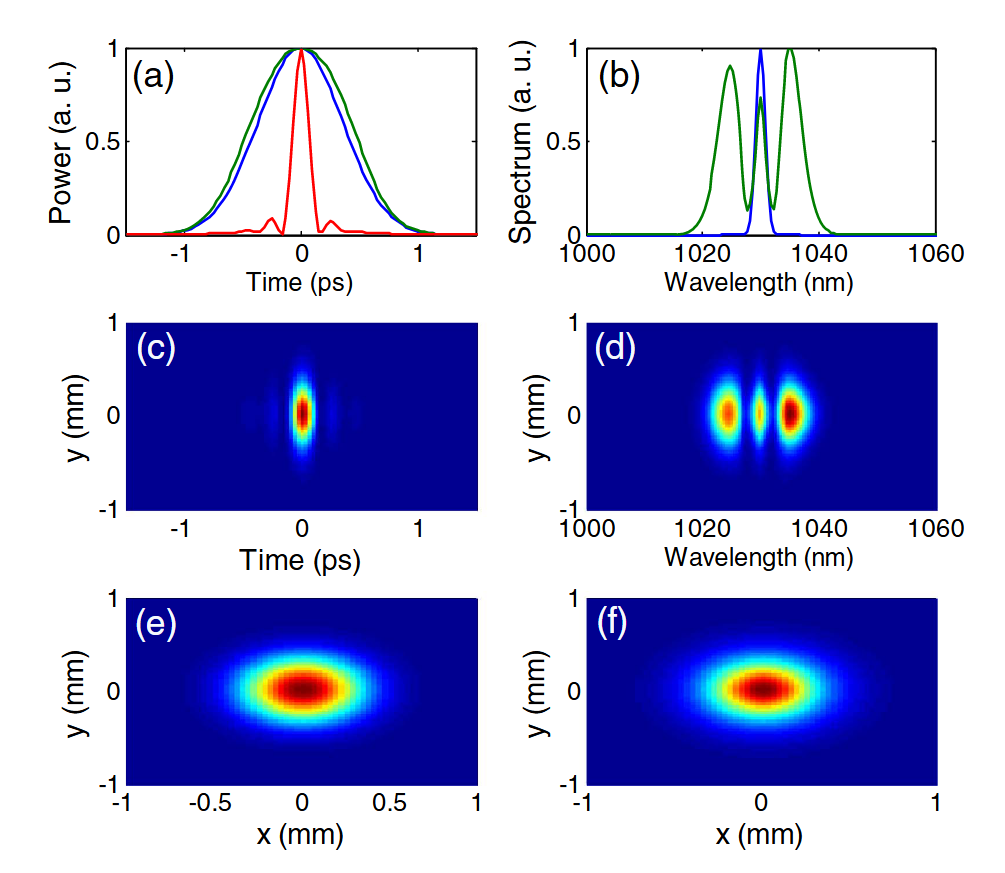
\includegraphics[width=0.5\textwidth]{p1.png}
    \caption{输入能量 30 $\mathrm{\mu J}$ 仿真: (a) 输入时间曲线（蓝色）、输出空间积分时间曲线在色散之前（绿色）和后（红色）； (b) 输入光谱（蓝色）和输出空间积分光谱（绿色）； (c) 压缩脉冲的时空分布； (d) 压缩脉冲的空间频谱轮廓； (e) 输入光束轮廓； (f) 输出时间积分光束轮廓. }\label{p2.2.1}
\end{figure}

结果如图 \ref{p2.2.1} 所示, 与实验非常吻合. 

· 输出 160 fs压缩脉冲（需要引入 $-30000\mathrm{fs^2}$的群延迟色散）

· 出色的频谱和时间均匀性

· 仿真计算 B 积分的轴上值为 19 rad, 与文献报告的估计值 5 $\pi$ 匹配. 

在输出光束轮廓上可以看到轻微光晕的出现以及输出光束尺寸的减小, 这表明每往返积累 ~1 rad 的 B 积分处于使用此设置不引入时空畸变的极限. 

\begin{figure}[h]
    \centering
    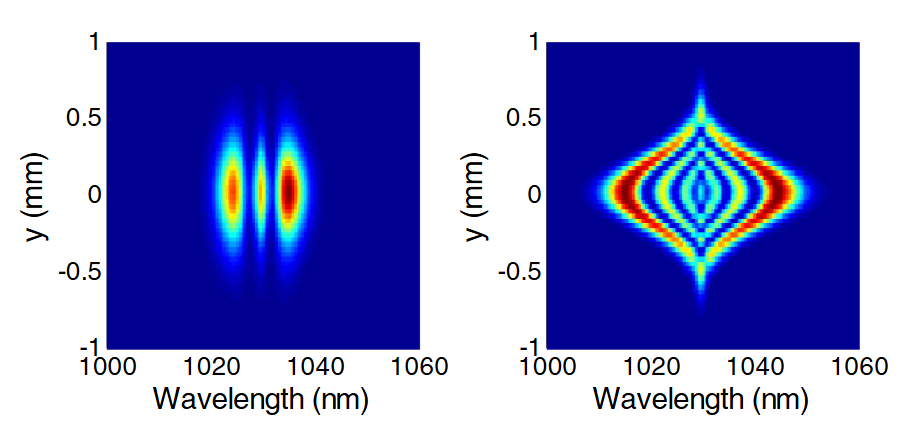
\includegraphics[width=0.4\textwidth]{p2.png}
    \caption{空间频谱分布比较: 腔体情况（左）; 一个平面中累积相同轴上 B 积分的脉冲（右）. }\label{p2.2.2}
\end{figure}

为说明腔的均匀化作用, 图 \ref{p2.2.2} 显示了上面获得的光谱空间分布, 与相同脉冲在单个平面中经历相同 B 积分的情况进行比较, 这接近于单级块体非线性压缩系统中发生的情况, 其中非线性晶体长度与输入准直光束的瑞利范围相比较小. 在这种情况下获得的强光谱空间耦合是显而易见的, 光谱展宽直接取决于横向空间强度. 

对后者, 在光束中心处观察到的光谱展宽对应于在腔体情况下观察到的等效 B 积分的两倍, 而由于强度空间上服从高斯分布, 它在光束边缘可以忽略不计. 相比之下, MPC在整个光束上重新分布这种非线性相位, 其过程类似于波导中发生的情况, 从而产生将累积 B 积分减半的有效面积, 如下式所示:
\begin{equation}
    B_\mathrm{roundtrip}=4\frac{2\pi n_2P_\mathrm{peak}}{ \lambda }\int_0^{L/2}\frac{1}{A_\mathrm{eff}(z)}\:\mathrm{d}z
    \label{eq:2.2.1}
\end{equation}

然后该模型以 40 $\mathrm{\mu J}$ 的输入能量运行, 以重现 Sartorius Thomas的工作\cite{schulteNonlinearPulseCompression2016} 中观察到的快速退化. 

\begin{figure}[h]
    \centering
    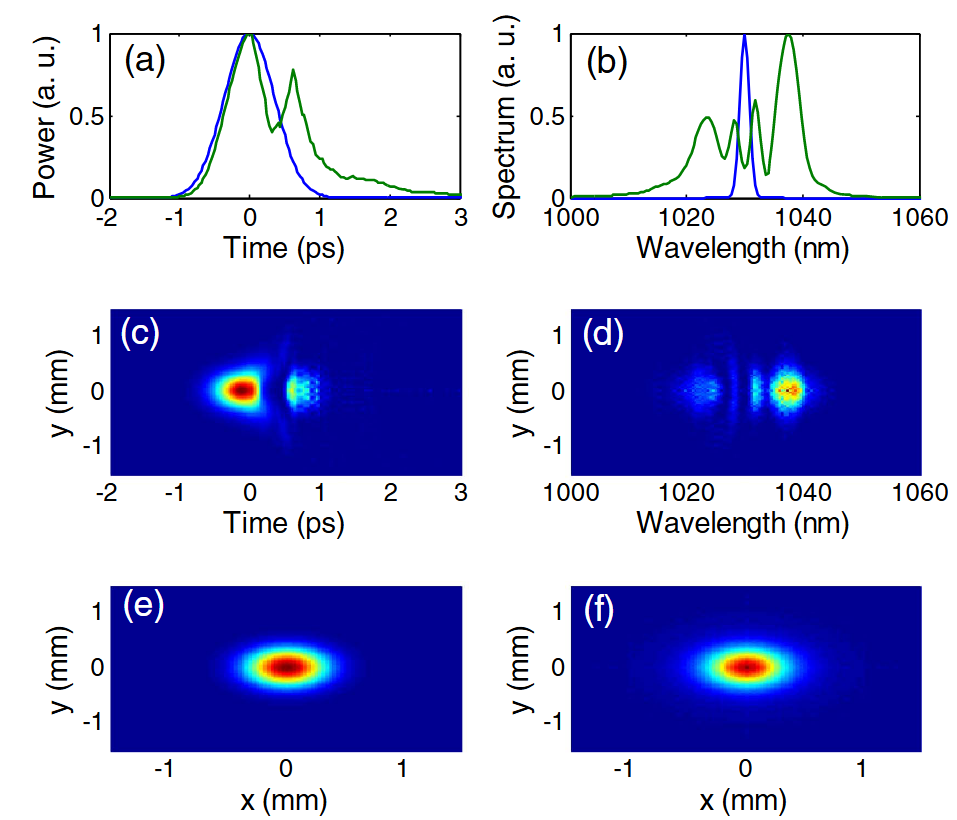
\includegraphics[width=0.4\textwidth]{p3.png}
    \caption{输入能量 40 $\mathrm{\mu J}$ 仿真结果: (a) 输入时间分布（蓝色）、色散前输出的空间积分时间分布（绿色）； (b) 输入光谱（蓝色）和输出空间积分光谱（绿色）； (c) 腔输出的时空分布； (d) 腔输出空间光谱分布； (e) 输入光束轮廓； (f) 输出的时间积分光束轮廓. }\label{p2.2.3}
\end{figure}

如图 \ref{p2.2.3} 所示, 脉冲无法再被压缩, 这表明我们的模型再现了空腔中空间均匀化过程的物理原理. 

图 \ref{p2.2.3}（b）所示光谱在形状和宽度均与报告实验结果匹配, 但并未完全再现. 这可归因于在发生快速光束衰减的能量范围内, 输出脉冲非常敏感地依赖于输入条件（例如能量和脉冲形状）. 另一种可能是, 由于存在显着的时空耦合, 实际中测量频谱的过程可能会对结果产生影响. 

作者对图 \ref{p2.2.3}(a) 中时间分布的解释为：时域上脉冲峰中心、高强度部分经历强烈的自聚焦并远离光束中心辐射, 如时空图中清楚展示的. 该光晕的一部分可以积累较大的群延迟, 形成延迟的时域上的翼以及在脉冲后沿观察到的干涉结构. 

\begin{figure}[h]
    \centering
    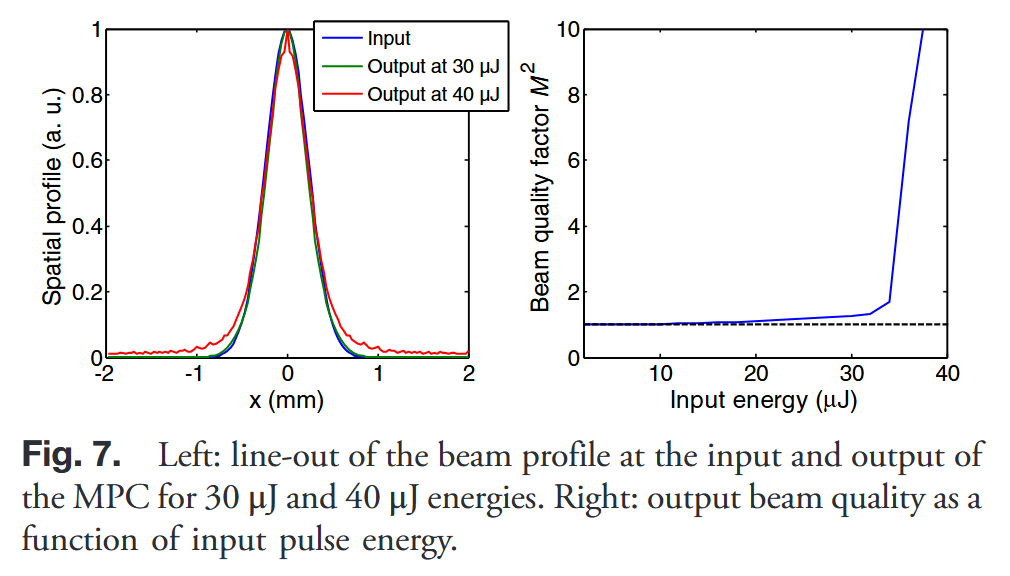
\includegraphics[width=0.4\textwidth]{p4.png}
    \caption{左图：30 $\mathrm{\mu J}$ 和 40 $\mathrm{\mu J}$ 能量的 MPC 输入和输出光束轮廓线; 右图：输出光束质量与输入能量关系}\label{p2.2.4}
\end{figure}

作者为进一步说明模拟捕获了实验观察到的在 30–40 $\mathrm{\mu J}$ 能量范围光束质量快速下降的情形, 图 \ref{p2.2.4}（左图）显示了 30 $\mathrm{\mu J}$ 和 40 $\mathrm{\mu J}$ 能量下腔体输入和输出的空间轮廓. 很明显, 很大一部分能量在 40 $\mathrm{\mu J}$ 的宽光晕中散发, 正如在单级块体材料的非线性压缩中通常观察到的. 作者计算了 MPC 输出的 $\mathrm{M_2}$ 参数（随时间变化的平均值）作为输入能量的函数. \ref{p2.2.4}（右图）清楚地显示了 35 $\mathrm{\mu J}$ 能量附近光束质量的快速下降, 与实验观察结果非常一致. 

\subsection{Nonlinear Compression in Gas-Filled MPCs}

模拟类似于 L. Lavenu的工作\cite{lavenuHighenergyFewcycleYbdoped2017}中描述的高能超短 Yb 掺杂光纤放大器在充气 MPC 中的压缩. 选择参数以在电离阈值和反射镜损坏阈值的安全区域内操作, 参数如下：

· 输入脉冲持续时间 150 fs, 脉冲能量 200 $\mathrm{\mu J}$, 

· 腔长 300 mm, 20 通, 腔中的非线性折射率为 $5\times 10^{−23} \mathrm{m^2∕W}$, 对应于 1 bar 的氙气或 5 bar 的氩气. 

· 反射镜曲率半径 300 mm, 无反射镜色散, 

相较前一案例, 能量几乎大一数量级, 且初始脉冲持续时间短得多, 目标是评估是否可以使用充气 MPC 来使用毛细管达到 L. Lavenu的工作\cite{lavenuHighenergyFewcycleYbdoped2017} 中描述的少周期范围, 同时提供鲁棒性并能方便地扩展到更高输入能量. 

\begin{figure}[h]
    \centering
    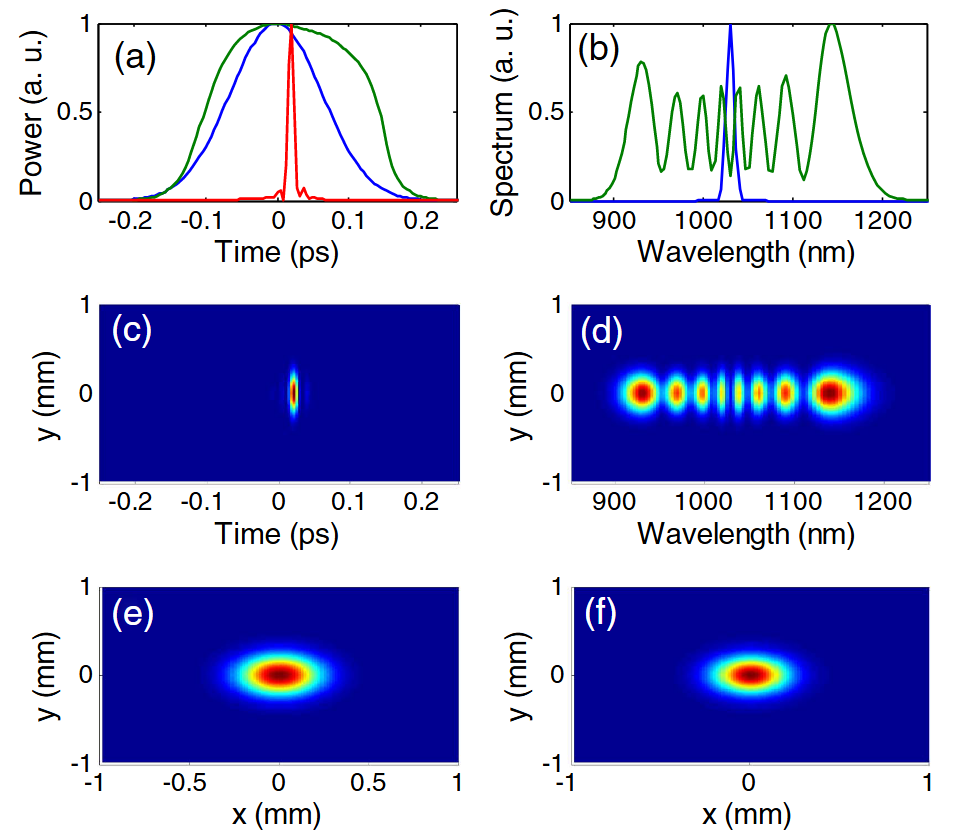
\includegraphics[width=0.4\textwidth]{p5.png}
    \caption{仿真结果: (a) 输入时间剖面（蓝色）, 输出空间积分时间剖面在色散之前（绿色）和之后（红色）； (b) 输入光谱（蓝色）和输出空间积分光谱（绿色）； (c) 压缩脉冲的时空分布； (d) 压缩脉冲的空间频谱轮廓； (e) 输入光束轮廓； (f) 输出时间积分光束轮廓. }\label{p2.3.1}
\end{figure}

模拟结果如图 \ref{p2.3.1} , MPC 能够压缩脉冲至 11 fs, 对应波长 1.03 $\mathrm{\mu m}$ 下 3.6 个光学周期, 同时保持极佳的输出光束质量. MPC技术构成了一极其通用的架构, 可在能量和脉宽度方面广泛的输入参数范围内使用. 

为进一步探索MPC的能量缩放, 现在将相同的模型应用于对应未来可能的基于高能二极管泵浦 $\mathrm{Yb:CaF_2}$ 系统, 即 $E_{\mathrm{in}}=500 \mathrm{mJ}$ 和 $\Delta \tau= 500 \mathrm{fs}$. 为避免电离和镜面损坏需要使用米级腔体:

· 6 m长, 镜面曲率半径为5 m, 接近共焦情况. 

· 为了远低于自聚焦阈值运行, 非线性参数调低至 $5 \times 10^{−26} \mathrm{m^2∕W}$, 约相当于 50 mbar 的Ne气. 

· 15次往返30通

\begin{figure}[h]
    \centering
    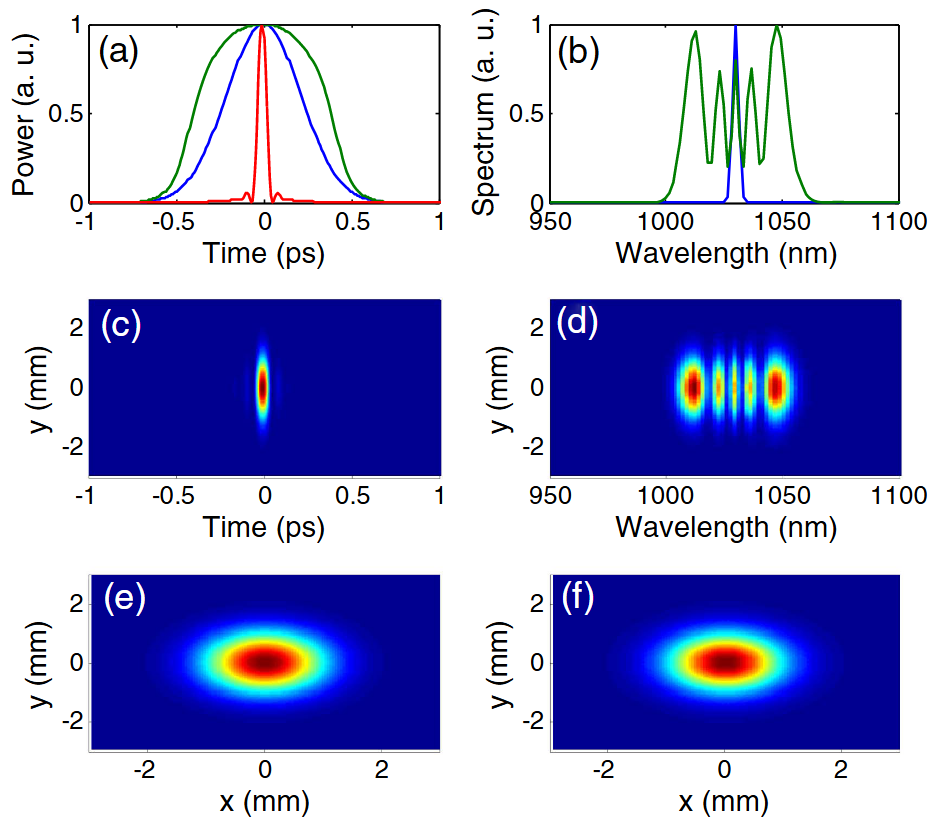
\includegraphics[width=0.4\textwidth]{p6.png}
    \caption{对应于高能块体 Yb:CaF2 系统的参数的仿真结果: (a) 输入时间剖面（蓝色）、输出空间积分时间剖面在色散之前（绿色）和之后（红色）； (b) 输入光谱（蓝色）和输出空间积分光谱（绿色）； (c) 压缩脉冲的时空分布； (d) 压缩脉冲的空间频谱轮廓； (e) 输入光束轮廓； (f) 输出时间积分光束轮廓. }\label{p2.3.2}
\end{figure}

输出脉冲空间质量良好, 且可压缩至 53 fs, 表明MPC技术原则上适用于太瓦激光系统. 

\subsection{Influence of Cavity Geometry on Space–Time Couplings}

作者为了更深入地了解设置对 MPC 参数的性能依赖性, 并从图 \ref{p2.3.1} 中描述的对应于光纤放大器的仿真操作点开始, 现在研究在固定曲率半径下压缩比和时空耦合作为非线性和腔长的函数. 为了充分探索参数可能, 作者不将 MPC 几何参数限制在避免镜面损坏和电离的情形. 

为了量化时空耦合, 作者引入了一个度量. 第一步是定义光束尺寸 $\Delta r(t)$ 和焦散 $\Delta f(t)$ 为二阶矩的平方根
\begin{equation}
    r=\sqrt{x^2+y^2},\quad f=\sqrt{f_{x}^{2}+f_{y}^{2}}
    \label{eq:2.4.1}
\end{equation}
分别是时间的函数. 

然后可以计算与时间相关的光束参数乘积
\begin{equation}
    \mathrm{BPP}(t)=\Delta r(t)\Delta f(t)
    \label{eq:2.4.2}
\end{equation}

然后, 时空耦合度量由BPP 随时间变化的平均值定义为 BPP 的标准偏差
\begin{equation}
    \mathrm{STC}=\sigma_\mathrm{BPP}/\langle\mathrm{BPP}\rangle 
    \label{eq:2.4.3}
\end{equation}

换言之, 当光束质量作为时间的函数为恒定值时, STC=0, 并且该值随着光束的空间属性越来越依赖于所考虑的时间值而增加. 任意定义的 STC 阈值低于 0.1 表明空间属性大多与时间无关, 从而在输出处产生可用的光束. 

\begin{figure}[h]
    \centering
    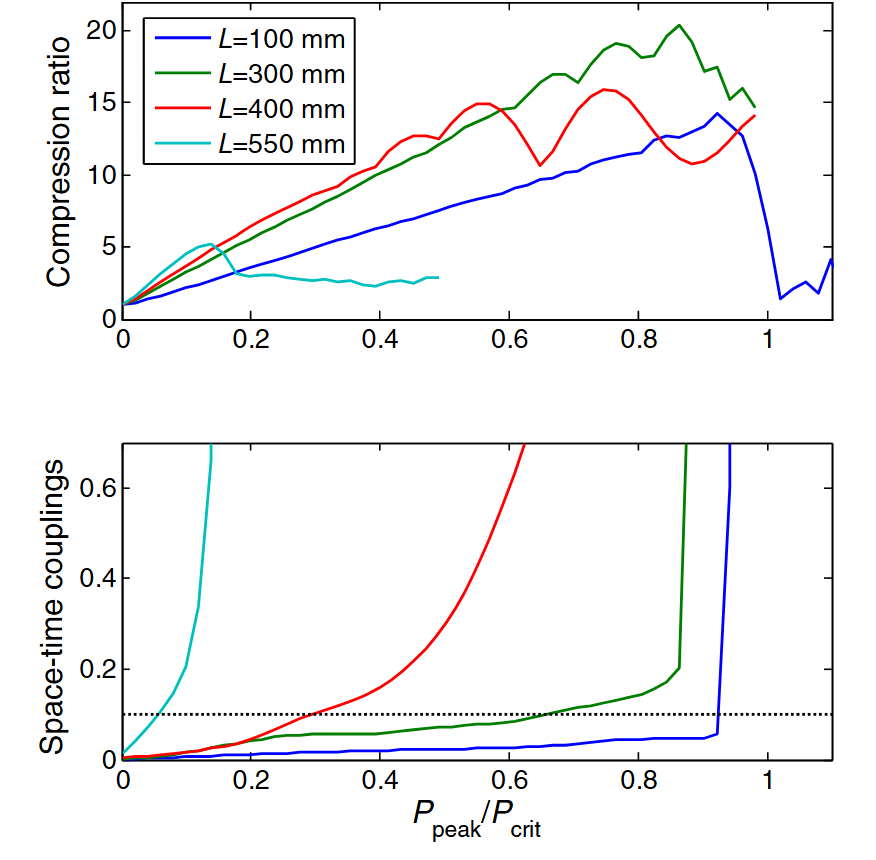
\includegraphics[width=0.4\textwidth]{p7.png}
    \caption{对于固定曲率半径 R=300 mm 的不同 MPC 长度, 压缩比（顶部）和时空耦合（底部）作为 $P_{\mathrm{peak}}∕P_{\mathrm{crit}}$ 比率的函数. 虚线表示STC=0.1. }\label{p2.4.1}
\end{figure}

图 \ref{p2.4.1} 展示了压缩比（定义为压缩峰值功率与输入峰值功率之比）以及时空耦合度量（用比率 $P_{\mathrm{peak}}∕P_{\mathrm{crit}}$ 表示）随 $n_2$ 增加的变化. 其他参数保持与图 \ref{p2.3.1} 相同. 

对于 $n_2$ 的每个值, 都通过在 MPC 的输出处添加二次空间无关的频谱相位来优化压缩. 

· 正如分析结果所预期, 随 $n_2$ 增加, 更长的 MPC 压缩比最初增加得更快, 由于每次往返累积 B 积分更大. 

· 但最长的MPC靠近同心稳定边缘, 会引起时空耦合的快速增加, 且不可能以大于5的功率压缩比压缩脉冲. 

图片直观地表明: 这种情况下, 非线性相位主要累积在束腰处, 在连续往返后成像到自身上, 从而允许像差累积, 而不是 SPM 的空间均匀化. 

总而言之, 短的, 共焦 MPC 都可以将脉冲压缩 10 到 15 倍, 同时保持较低的时空耦合. 随 MPC 长度增加, 与输出端可接受的时空耦合相对应的 $P_{\mathrm{peak}}∕P_{\mathrm{crit}}$ 值会减小. 

\section{总结}

1. 学习了解了MPC仿真的一些方法概述.

· 3D模型

· 2D模型

· 1D模型

2. 作者仿真的使用和详细的分析也可为未来作为参考.

3. 作者引入了时空耦合的量化度量, 这一方法和参数或许可以借鉴.
%--------------------  插入参考文献  --------------------%

\newpage

\clearpage           %%%  “目录”中显示的页码正确, 需要添加 \clearpage
\phantomsection      %%   “目录”中的链接能正确跳转, 需要添加 \phantomsection
\addcontentsline{toc}{section}{参考文献}   %向目录中添加条目, 以章的名义

\bibliography{ref}

\end{document}